\documentclass[11pt,a4paper]{article}
\usepackage[T1]{fontenc}
\usepackage{lmodern,amsmath,amssymb,amsthm,mathtools}
\usepackage[margin=25mm,headheight=15pt]{geometry}
\usepackage{graphicx,booktabs,longtable,array,tabularx}
\usepackage[dvipsnames]{xcolor}
\usepackage{microtype,enumitem,fancyhdr}
\usepackage[colorlinks=true,linkcolor=MidnightBlue,citecolor=MidnightBlue,urlcolor=MidnightBlue]{hyperref}
\usepackage{bookmark}
\hypersetup{pdftitle={Transient Collective Turning and Coherent Relaxation in the Native Triad},pdfauthor={Hilmir Frimann Halldorsson},pdfsubject={Author-authorized repository research edition v0.1, 28 October 2026; project-internal review complete}}
\setlength{\parskip}{4pt}
\setlength{\parindent}{0pt}
\setlength{\emergencystretch}{3em}
\setlist{itemsep=2pt,topsep=4pt}
\pagestyle{fancy}\fancyhf{}
\fancyhead[L]{\small Collective turning and coherent relaxation}
\fancyhead[R]{\small Research edition v0.1}
\fancyfoot[C]{\thepage}
\renewcommand{\headrulewidth}{0.3pt}
\numberwithin{equation}{section}
\newtheorem{theorem}{Theorem}[section]
\newtheorem{proposition}[theorem]{Proposition}
\newtheorem{lemma}[theorem]{Lemma}
\theoremstyle{remark}\newtheorem{remark}[theorem]{Remark}
\newcommand{\C}{\mathbb C}\newcommand{\R}{\mathbb R}
\newcommand{\one}{\mathbf1}\newcommand{\eps}{\varepsilon}
\newcommand{\re}{\operatorname{Re}}\newcommand{\im}{\operatorname{Im}}
\newcommand{\Argz}{\operatorname{Arg}_0}
\newcommand{\diag}{\operatorname{diag}}
\newcommand{\pin}{ad8a6e88b4a78d8b1955b34d5ff80b6c21713ade}
\newcolumntype{Y}{>{\raggedright\arraybackslash}X}
\newcolumntype{L}[1]{>{\raggedright\arraybackslash}p{#1}}
\begin{document}
\hypersetup{pageanchor=false}
\begin{titlepage}
\vspace*{8mm}
{\small\color{MidnightBlue} TRI-OCTAGON MATHEMATICAL RESEARCH\par}
\vspace{7mm}
{\LARGE\bfseries Transient Collective Turning and Coherent Relaxation in the Native Triad\par}
\vspace{7mm}
{\large Hilmir Fr\'imann Halld\'orsson\par}
\vspace{3mm}
{\normalsize Repository research edition v0.1 --- 28 October 2026\par}
\vspace{5mm}
{\small\bfseries Author-authorized repository research edition v0.1. GPT project-internal scientific review and author review completed. No external peer review is claimed.\par}
\vspace{5mm}
\begin{abstract}
We synthesize a completed bounded investigation of the existing native Tri-Octagon recurrence. A retained, rigorously enclosed two-step example shows that the complex channel mean can turn while an amplitude ratio changes. An exact matched comparison with synchronization disabled then isolates delayed graph influence: graph redistribution cancels from the first mean step but changes the second through the nonlinear onsite response. Its dependence on graph strength is an exact cubic polynomial. At the prescribed comparison point the second increment changes direction even though the signed-turn statistic decreases. Separately, for the full ordered map at the same nonzero synchronization strength, an explicit annulus-and-sector domain is invariant. Ordinary phase separations contract; dispersion obeys a contraction-with-mismatch estimate; and every state in that domain converges to a unique positive unequal amplitude profile in a specified cube, up to an initial-state-dependent limiting common phase. The mean settles, residual amplitude spread is positive, and the signed-area observables decay to zero. The turning entrance lies outside this domain, so these results do not establish a single trajectory that turns, enters the domain, and settles. We distinguish the author's uncertain historical recollection, exact algebra, analytical proofs, retained computational certificates, and mathematical comparisons with physical force laws. No new simulation, root solve, kernel change, or physical identification is used.
\end{abstract}
\vfill
{\small Mathematical source baseline: \nolinkurl{\pin}.\\
Author's observation and programme: Hilmir Fr\'imann Halld\'orsson. GPT supplied scientific steering and project-internal review of the preceding results and the assembled manuscript. Codex assisted with mathematical derivation, retained checking, and this manuscript's preparation. GPT scientific review and author review were completed on 28 October 2026; no external peer review is claimed.}
\end{titlepage}
\pagenumbering{roman}\hypersetup{pageanchor=true}
\setcounter{tocdepth}{1}
\begingroup\small\setlength{\parskip}{0pt}\tableofcontents\endgroup
\clearpage\pagenumbering{arabic}

\section{The observation and the mathematical questions}\label{sec:overview}

The investigation began with the author's recollection of a display: one component seemed to drift, two seemed to rotate around one another, and the combined size of those two seemed equal to the first. Their interaction appeared capable of producing a newly directed path. The later clarification was more specific about the remembered numbers and less specific about their identity: there had been three very small numbers, two apparently adding to the third; ``size'' meant numerical magnitude; and they appeared to travel toward the center. The author explicitly expressed uncertainty about this memory. These statements are retained as a research lead, not as a verified physical observation or a recovered historical formula. The preparation order records the recollection in this form \cite{order}.

The mathematical question that can be answered without recovering the display is whether the existing recurrence permits its collective complex mean to change direction while internal shape changes. A second question asks whether internal graph redistribution can cause such a change, even though the graph term has zero channel sum. A third asks what the full map does in an explicit region where amplitudes remain moderate and ordinary phases are already close. These questions have different evidential requirements. A single certified example answers an existence question; a matched comparison isolates a coefficient's effect; a theorem over a stated domain supplies a long-time conclusion.

The answer to the first question is positive. Three retained states give two noncollinear collective increments, while a channel intensity ratio changes by an exact amount. The answer to the second is also positive on the specified phase-off comparison: the graph changes the direction of the second mean increment through the later onsite response. This effect is delayed because the first phase-off mean step is independent of the graph coefficient. It need not increase the signed area formed by consecutive increments. In the recorded comparison, that area decreases while the second increment rotates and shortens.

The answer to the third question is convergence. Within a stated annulus and narrow ordinary phase sector, the full ordered map approaches a fixed circle of unequal aligned states. Different initial states can select different points on that circle. Their limiting amplitude profile is the same, their ordinary relative phases vanish, and their signed-area observables vanish. Unequal coefficients leave a positive amplitude spread even though phase alignment becomes exact in the limit.

\textbf{These are separate results.} The turning entrance has moduli $\sqrt2,\sqrt2,\sqrt5$, outside the convergence annulus. No capture of that entrance into the invariant region has been proved. The manuscript neither draws nor implies a connecting trajectory. The shared coefficients make the contrast informative, but do not supply the missing capture argument.

\begin{table}[htbp]\centering\small
\caption{Recollection and mathematical candidates. No row identifies the historical display.}
\begin{tabularx}{\textwidth}{@{}L{.26\textwidth}YY@{}}\toprule
Author-supplied lead & Candidate examined & Identification status\\\midrule
One drifting component; two apparently rotating & Complex mean and changing internal shape & A constructed turning witness exists; no recovered display correspondence.\\
Two small magnitudes apparently sum to a third & Three zero-sum graph corrections; separately, three zero-sum real phase kicks & Both balances are exact. Magnitude addition needs additional conditions. Neither is historically identified.\\
Apparent motion toward a center & Graph correction toward the channel mean; finite-domain relaxation & Mathematical statements in state space, without an identified physical center.\\
Uncertain numerical memory & Particular channels, relative modes, forces, or SRG constants & No assignment to these quantities has been established.\\\bottomrule
\end{tabularx}
\end{table}

This presentation consolidates completed results rather than opening a new investigation. Its propositions received project-internal mathematical discussion before drafting. The assembled manuscript subsequently completed GPT scientific review and author review and is authorized as this repository research edition. Accepted source papers provide the recurrence, geometric attachments, local branches, and related dynamical results. The distinctions between those inherited results and the completed propositions are recorded in \path{CLAIM_SOURCE_MAP.md}.

\section{Native map, notation, and observable spaces}\label{sec:map}

Let $\Omega_n\in\C^3$ have channels $A,B,C$, and let $\eps,g,\lambda,k_i$ be real. With the negative-semidefinite graph convention
\begin{equation}
L_3=\one\one^T-3I=
\begin{pmatrix}-2&1&1\\1&-2&1\\1&1&-2\end{pmatrix},
\end{equation}
the native update is
\begin{align}
v_{i,n}&=\Omega_{i,n}+\eps\Omega_{i,n}(k_i-|\Omega_{i,n}|^2)
                   +g(L_3\Omega_n)_i,\label{eq:pre}\\
\delta_{i,n}&=\lambda\sum_{j\ne i}\sin3(\Argz v_{j,n}-\Argz v_{i,n}),\label{eq:kicks}\\
\Omega_{i,n+1}&=v_{i,n}e^{i\delta_{i,n}}.\label{eq:post}
\end{align}
Every kick uses the same prestage $v_n$. Updating one phase and using it to calculate another kick would define a different map. The native convention is $\Argz(0)=0$; a zero prestage component stays zero after multiplication. There is no amplitude normalization. These definitions agree with the implementation and Paper A's ordered recurrence \cite{kernel,paperA}.

The formula is globally defined under its zero convention, but phase coordinates and smooth common-phase equivariance require care. Throughout arguments using such coordinates we work on regular states with nonzero relevant prestages. The witness certificate checks this regularity, and the invariant domain proves it for all subsequent steps. Away from zeros, simultaneous multiplication by $e^{i\alpha}$ commutes with the map. Conjugation commutes with the real-parameter recurrence and reverses its phase kicks. At the zero stratum, unrestricted common-phase quotient claims would conflict with the native convention, as the accepted observable-closure analysis explicitly shows \cite{closure}.

Define the mean, projection, relative state, and dispersion by
\begin{equation}
m=\frac13\one^T\Omega,\qquad P=I-\frac13\one\one^T,
\qquad\eta=P\Omega=\Omega-m\one,\qquad E=\|\eta\|_2.
\label{eq:mean}
\end{equation}
The identity
\begin{equation}
E^2=\frac13\sum_{i<j}|\Omega_i-\Omega_j|^2\label{eq:pairspread}
\end{equation}
is useful because the synchronizer changes phases but preserves each modulus. It follows by expanding both sides, or from orthogonal projection onto the complement of the common channel vector.

For $x=\re\Omega$ and $y=\im\Omega$, Paper G defines
\begin{gather}
C=x\times y=(x_By_C-x_Cy_B,\ x_Cy_A-x_Ay_C,\ x_Ay_B-x_By_A)^T,\label{eq:area}\\
T=\begin{pmatrix}-1/2&1&-1/2\\-\sqrt3/2&0&\sqrt3/2\\0&0&0\end{pmatrix},
\qquad W=TC,\qquad\Gamma=\one^TC.\label{eq:attach}
\end{gather}
There is no factor $1/2$: the entries are signed parallelogram areas. $C$ is a vector in channel-index space. $T$ attaches it to the fixed ambient geometry, producing the horizontal axial observable $W$; $\Gamma$ retains the complementary common component. In particular $T^TT=(3/2)P$. These are passive functions of the state, not extra evolved variables or feedback forces \cite{paperG,closure}. Common phase leaves them unchanged, while conjugation reverses their signs.

\begin{longtable}{@{}p{.21\textwidth}p{.74\textwidth}@{}}
\caption{Notation and correspondence with the source reports.}\label{tab:notation}\\\toprule
Symbol & Meaning and distinction\\\midrule\endfirsthead
\toprule Symbol & Meaning and distinction\\\midrule\endhead
$m,\eta,E$ & Complex channel mean, relative state, and its Euclidean norm. $m$ is not a mass.\\
$\kappa_i=k_i-\bar k$ & Coefficient heterogeneity; distinct from relative state $\eta$. The drift source uses $\eta$ for a coefficient parameter; it is renamed $a_{\rm het}$ when needed here.\\
$B_n,S_n$ & Onsite and synchronization contributions to the mean increment. $S_n$ is not dispersion or a Gram matrix.\\
$G_{\rm R}=xx^T+yy^T$ & Real Gram matrix, denoted $S$ in Paper G and $S_G$ in the closure source. It is distinct from $E^2$.\\
$C,W,\Gamma$ & Channel-area vector and its fixed attachments. $C_{\rm disp}$ is a scalar residual bound, not $C$.\\
$P;\ P_1,P_2,P_3$ & Orthogonal channel projector; separately, complex coefficients of the delayed-response polynomial.\\
$s,t(g);\ K,J,R,Q$ & Mean increments and signed cross/dot diagnostics for the phase-off comparison. $Q$ in $Q(g)$ is a scalar diagnostic; the cube $\mathcal Q$ is distinct.\\
$\Delta_n,c,\beta,q$ & Ordinary phase width and three distinct contraction bounds: phase, aligned amplitude, and dispersion with mismatch.\\
$M_a,q_{\rm el},\tau$ & Physical mass, charge, and time used only in the external comparison.\\\bottomrule
\end{longtable}

The implementation has no physical clock, mass or charge assignment, or geometry-feedback law \cite{kernel}. Consequently the complex plane used for $m$ is a state-coordinate plane. A spatial interpretation would require additional, separately justified correspondences rather than a change of axis labels.

\section{Exact accounting of the collective increment}\label{sec:account}

The graph is conservative with respect to the unweighted channel sum:
\begin{equation}
\one^TL_3=0.
\end{equation}
Taking the mean of \eqref{eq:pre} and then of \eqref{eq:post} gives the exact decomposition
\begin{align}
m_{n+1}-m_n&=B_n+S_n,\label{eq:budget}\\
B_n&=\frac\eps3\sum_i\Omega_{i,n}(k_i-|\Omega_{i,n}|^2),\\
S_n&=\frac13\sum_i v_{i,n}(e^{i\delta_{i,n}}-1).
\end{align}
No first-order approximation of the phase exponential has been made. The individual graph corrections sum to zero, so they contribute no direct term to the prestage mean. The onsite contribution still depends on the entire state, not just its mean: unequal channel magnitudes and phases enter its cubic factors.

Three different statements must be kept apart. First, the explicit graph sum cancels from the prestage mean for any state and any real $g$. Second, in a matched comparison with the same initial state, $\eps$, and $k$, and with $\lambda=0$, the first complete mean step is independent of $g$, because then $S_0=0$. Third, at nonzero $\lambda$, changing $g$ changes $v_0$ and can immediately change $S_0$. Direct cancellation is therefore not independence of the complete mean dynamics from graph coupling.

Even with synchronization off, graph redistribution changes the individual first states. The next onsite evaluation samples those changed states through $z\mapsto z(k_i-|z|^2)$. Averaging that nonlinear response need not cancel the earlier redistribution. Section~\ref{sec:delayed} makes this mechanism exact and distinguishes it from the existence of turning alone.

The decomposition also prevents an overly simple assignment of motion to one operation. $B_n$ and $S_n$ add as complex vectors, with possible reinforcement or cancellation; their directions are not fixed forces. Changing an operation can change the states supplied to all later operations. Thus a stage budget describes the realized update, whereas a matched coefficient comparison describes a controlled difference between two maps. Both are useful, but they answer different causal questions.

\section{A retained full-map turning witness}\label{sec:witness}

The documented parameter point is
\begin{equation}
\eps=\frac1{10},\quad g=\frac1{60},\quad\lambda=\frac1{300},
\quad k=(999/1000,1,1001/1000).\label{eq:parameters}
\end{equation}
It is the point $h=1/10$, $a_{\rm het}=1/1000$ in the already documented family $(\eps,g,\lambda)=h(1,1/6,1/30)$, $k=(1-a_{\rm het},1,1+a_{\rm het})$ \cite[labels D2 and D41]{drift}. This parameter point was fixed before evaluating the witness; the constructed entrance is
\begin{equation}
\Omega_0=(1+i,1+i,1-2i),\qquad m_0=1.\label{eq:entrance}
\end{equation}
It is a mathematical example, not a recovered version of the author's remembered small numbers.

Define the signed two-step turn
\begin{equation}
K_m=\im\!\left[\overline{(m_1-m_0)}(m_2-m_1)\right].\label{eq:turn}
\end{equation}
For nonzero increments this equals the product of their lengths times the sine of their oriented angle. It establishes noncollinearity when nonzero, but it is not a pure angle measure.

The retained interval certificate supplies the following closed enclosures \cite{turnreceipt}. Each pair of endpoints bounds the exact-map quantity; the values are not raw floating trajectory output.
\begin{table}[htbp]\centering\small
\caption{Certified collective increments for the full map.}
\begin{tabular}{@{}lll@{}}
\toprule
Step & $\Re\Delta m$ & $\Im\Delta m$ \\
\midrule
0 to 1 & $[-0.2031076834, -0.2031076833]$ & $[0.2003797848, 0.2003797849]$ \\
1 to 2 & $[-0.0463219019, -0.0463219018]$ & $[-0.0088332477, -0.0088332476]$ \\
\bottomrule
\end{tabular}

\end{table}

In particular,
\begin{equation}
0.0110760731\le K_m\le0.0110760732,\label{eq:certturn}
\end{equation}
which excludes zero. The two increments turn while internal shape changes. The first prestage is exactly
\begin{equation}
v_0=\left(\frac{8999+8499i}{10000},\ \frac{9}{10}+\frac{17}{20}i,
\ \frac{6001-11002i}{10000}\right).
\end{equation}
Since synchronization preserves moduli,
\begin{equation}
\frac{|\Omega_{A,0}|^2}{|\Omega_{C,0}|^2}=\frac25,
\qquad
\frac{|\Omega_{A,1}|^2}{|\Omega_{C,1}|^2}
=\frac{153215002}{157056005}\ne\frac25.\label{eq:ratio}
\end{equation}
A rigid common-phase relative equilibrium preserves every component intensity and every such ratio. Equation~\eqref{eq:ratio} therefore rules out that explanation for this witness.

\begin{figure}[htbp]\centering
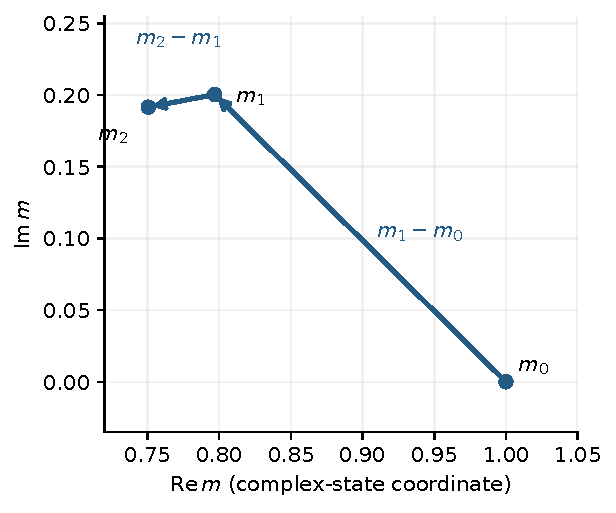
\includegraphics[width=.84\textwidth]{figures/mean_two_steps.pdf}
\caption{The retained three means, drawn using enclosure midpoints. Arrows show the two discrete increments only; no interpolating orbit is asserted. Axes are complex-state coordinates. The certificate, not the plot resolution, establishes the turn.}
\end{figure}

The existing attachment changes on the same states:
\begin{table}[htbp]\centering\small
\caption{Retained enclosures for the passive observable $W$; $W_z=0$ throughout.}
\begin{tabular}{@{}lll@{}}
\toprule
$n$ & $W_x$ & $W_y$ \\
\midrule
0 & $4.5000000000$ & $[2.5980762113, 2.5980762114]$ \\
1 & $[2.2459234658, 2.2459234659]$ & $[1.2967881135, 1.2967881136]$ \\
2 & $[1.8956060860, 1.8956060861]$ & $[1.0945688105, 1.0945688106]$ \\
\bottomrule
\end{tabular}

\end{table}

For example $C_0=(-3,3,0)$ and $W_0=(9/2,3\sqrt3/2,0)$. The disjoint later enclosures show a change in the attachment, without assigning it magnetic units or making it a source of the state update. Appendix~\ref{app:budgets} gives the retained onsite and synchronization mean contributions.

A single matched phase-off comparison at the same entrance, $\eps,g,k$, yields
\begin{equation}
K_m^{\rm off}=
\frac{3158587023292997}{300000000000000000}>0.\label{eq:offturn}
\end{equation}
Thus synchronization is not necessary for this witness's turning. This comparison alone does not establish the necessity of graph coupling or of unequal $k_i$. Turning is an output geometry; it does not by itself identify which mechanism produced it. Section~\ref{sec:delayed} uses the completed controlled graph comparison to establish a narrower mechanism statement.

Conjugating \eqref{eq:entrance} gives a handedness control with the same component intensities and the same initially real mean. Real-parameter conjugation equivariance conjugates both mean increments, reversing $K_m$, and sends $(C,W,\Gamma)$ to their negatives. No second numerical trajectory is needed. This is an exact symmetry control, not evidence that the sign is a magnetic field.

The retained checker used integer-endpoint outward-rounded arithmetic with denominator $2^{200}$. It evaluated phase sines through normalized complex products, and bounded the short-kick exponential by Taylor polynomials with explicit remainders. Every input, prestage, and output component in these two updates has modulus greater than one. The regularity and positivity claims belong to that existing finite certificate, which is included unchanged and was not rerun for this manuscript.

\section{Matched graph-coupling comparison on \texorpdfstring{$\lambda=0$}{lambda=0}}\label{sec:delayed}

This section holds the entrance, $\eps$, and $k$ fixed and varies only the real graph coefficient, with synchronization disabled. It does not transfer first-step independence from $g$ to the full nonzero-$\lambda$ map. Write
\begin{equation}
f_i(z)=z(k_i-|z|^2),\qquad
a_i=\Omega_{i,0}+\eps f_i(\Omega_{i,0}),\qquad d=L_3\Omega_0.
\end{equation}
The first state is $a+gd$, and $\sum_i d_i=0$. Thus $m_1(g)=\frac13\sum_i a_i$ is constant in $g$. The second graph sum also cancels directly, leaving
\begin{equation}
D(g):=m_2(g)-m_2(0)
=\frac\eps3\sum_i[f_i(a_i+gd_i)-f_i(a_i)].\label{eq:Ddef}
\end{equation}

\begin{proposition}[Exact delayed mean response]\label{prop:poly}
For fixed entrance, $\eps$, and real $k_i$, on the phase-off slice the response is exactly
\begin{equation}
D(g)=gP_1+g^2P_2+g^3P_3,\label{eq:poly}
\end{equation}
where, with $u_i=\re(\bar a_i d_i)$,
\begin{align}
P_1&=\frac\eps3\sum_i[(k_i-|a_i|^2)d_i-2u_i a_i],\label{eq:P1}\\
P_2&=-\frac\eps3\sum_i[2u_i d_i+|d_i|^2a_i],\label{eq:P2}\\
P_3&=-\frac\eps3\sum_i|d_i|^2d_i.\label{eq:P3}
\end{align}
There is no omitted remainder.
\end{proposition}
\begin{proof}
For real $g$,
\[
|a_i+gd_i|^2=|a_i|^2+2gu_i+g^2|d_i|^2.
\]
Multiplying by $a_i+gd_i$, subtracting the constant term, and inserting the result in \eqref{eq:Ddef} yields \eqref{eq:P1}--\eqref{eq:P3}. Terms of higher degree cannot arise from this cubic onsite map after the first affine dependence on $g$.
\end{proof}

The linear-$k$ contribution is confined to
\begin{equation}
P_{1,k}=\frac\eps3\sum_i k_i d_i,
\qquad P_{1,\rm cub}=P_1-P_{1,k}.
\end{equation}
Both $P_2$ and $P_3$ come from the cubic response. If the $k_i$ are equal, $P_{1,k}=0$, but this does not force the cubic coefficients to vanish. Conversely, nonzero coefficients can cancel at a particular nonzero $g$. The polynomial's coefficients and its value at one point are different assertions.

The first coefficient has a direct differential interpretation. For a complex direction $h$, treated as a vector in $\R^2$,
\begin{equation}
Df_i(a)[h]=(k_i-|a|^2)h-2a\re(\bar a h).\label{eq:realderivative}
\end{equation}
At $a\ne0$, its radial and tangential factors are respectively $k_i-3|a|^2$ and $k_i-|a|^2$. Thus the same redistribution can be weighted differently along and across a channel's current phase. This is a real directional derivative, not a holomorphic derivative: $|z|^2$ depends on $\bar z$. Summing these differently weighted responses is the mechanism by which an initially zero-sum graph displacement can acquire a nonzero mean effect one step later.

Define the directional diagnostics before using their signs:
\begin{align}
s&=m_1-m_0,&t(g)&=m_2(g)-m_1,\\
K(g)&=\im(\bar s\,t(g)),&J(g)&=K(g)-K(0),\label{eq:diagnostics}\\
R(g)&=\im(\overline{t(0)}t(g)),&Q(g)&=\re(\overline{t(0)}t(g)).
\end{align}
Here $J(g)=\im(\bar sD(g))$ and $R(g)=\im(\overline{t(0)}D(g))$. The former compares signed-turn statistics against the same first increment; the latter directly compares the directions of the two second increments. The dot product $Q$ resolves the acute-versus-obtuse distinction and detects reversals when the cross product vanishes.

At the prescribed comparison point $g_*=1/60$, the retained exact calculation gives
\begin{align}
s&=-\frac15+i\frac{1999}{10000},\\
t(0)&=-\frac{1596353944003}{30000000000000}
       -i\frac{39208493497}{7500000000000},\label{eq:t0}\\
t(g_*)&=-\frac{1300824689003}{30000000000000}
       -i\frac{23259936249}{2500000000000},\label{eq:tg}\\
D(g_*)&=\frac{59105851}{6000000000}
        -i\frac{122285261}{30000000000}.\label{eq:Dstar}
\end{align}
The sign conclusions are exact rational comparisons \cite{graphreceipt}:
\begin{align}
J(g_*)&=-\frac{69238491749}{60000000000000}<0,\\
R(g_*)&=\frac{241559586182149258723}{900000000000000000000000}>0,\\
Q(g_*)&=\frac{2120352001586073403391153}{900000000000000000000000000}>0.
\label{eq:signs}
\end{align}
Both second increments are nonzero. The positive cross and dot products establish an acute counterclockwise directional change from $t(0)$ to $t(g_*)$. Yet $K(g_*)<K(0)$, with both positive. The exact components also show $|\re t(g_*)|<0.044$, $|\im t(g_*)|<0.010$, and $|\re t(0)|>0.053$, so
\[
|t(g_*)|^2<0.044^2+0.010^2=0.002036
<0.053^2<|t(0)|^2.
\]
The changed second increment is shorter. A signed-turn statistic multiplies an angle factor by increment lengths; its decrease therefore cannot be interpreted as absence of directional response.

\begin{figure}[htbp]\centering
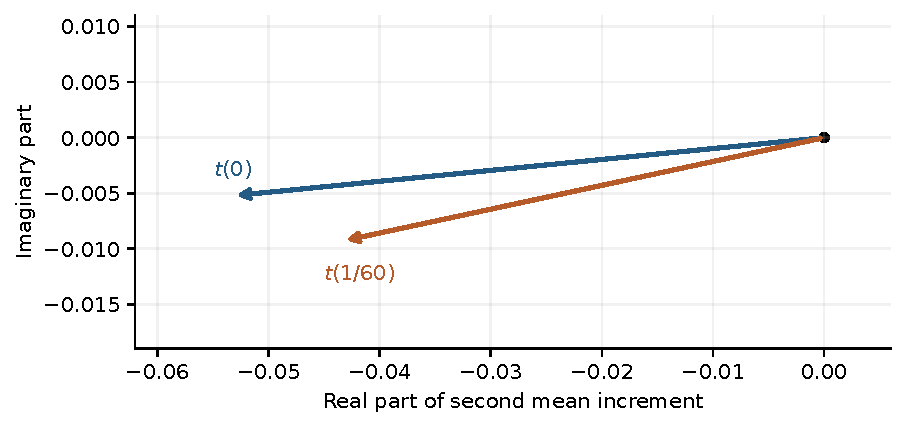
\includegraphics[width=.86\textwidth]{figures/matched_second_steps.pdf}
\caption{Matched phase-off second increments, drawn from the retained exact fractions. Graph coupling changes direction and shortens the vector. These are two comparison vectors with a common origin, not successive segments of a new trajectory.}
\end{figure}

Several qualifications are essential. If $s=0$, then $K$ and $J$ vanish without determining the direction of $t$. If either second increment is zero, its angle is undefined. For nonzero second increments, $R=0$ means collinearity: $Q>0$ means the same direction and $Q<0$ means reversal. A nonzero $D$ may have $J=0$ because its projection perpendicular to $s$ vanishes, and may have $R=0$ for a different reason. A vanished first coefficient is not a vanished response unless the remaining coefficients or their evaluated sum also vanish.

On a common real line $e^{i\alpha}\R^3$, the phase-off map keeps all states on that line; signed turns vanish even when magnitudes and signs change. If $d=0$, there is no first-step graph displacement, so this two-step delayed response is zero. If $\eps=0$, both phase-off mean increments vanish because only zero-sum graph redistribution remains. These conditions delimit the conclusion; the prescribed witness satisfies the nondegenerate comparisons explicitly. Restoring synchronization introduces its own nonlinear response and invalidates the first-step cancellation argument for the complete mean. No claim about its necessity is inferred from the phase-off polynomial.

\section{An invariant domain for the full ordered map}\label{sec:domain}

Return to all coefficients in \eqref{eq:parameters}, including $\lambda=1/300$. Let $\mathcal D$ consist of states with $0.9\le|\Omega_i|\le1.1$ and ordinary phases in one interval of width at most $D_0=\pi/12$. The interval may be rotated by any common angle. It is not an interval in phase modulo $2\pi/3$.

\subsection{The phase-stage lemma}
\begin{lemma}\label{lem:phase}
Suppose positive-modulus inputs have ordinary phases $\theta_i$ in an interval $[a,b]$ of width $D<\pi/6$, and $0\le\lambda\le1/9$. The simultaneous synchronizer preserves their ordering, keeps every phase in $[a,b]$, and satisfies
\begin{equation}
|\theta_i^+-\theta_j^+|\le(1-9\lambda\cos3D)|\theta_i-\theta_j|.
\label{eq:phaselemma}
\end{equation}
It does not increase dispersion $E$, even for unequal positive moduli.
\end{lemma}
\begin{proof}
For the fixed input phases define
\[
G(x)=x+\lambda\sum_{k=1}^3\sin3(\theta_k-x).
\]
The self term is zero at $x=\theta_i$, so $\theta_i^+=G(\theta_i)$. For $x\in[a,b]$,
\begin{equation}
0\le1-9\lambda\le G'(x)
=1-3\lambda\sum_k\cos3(\theta_k-x)
\le1-9\lambda\cos3D\le1.
\end{equation}
Monotonicity proves ordering. Since $G(a)\ge a$ and $G(b)\le b$, it also proves interval preservation. The mean-value theorem gives \eqref{eq:phaselemma}. Finally, for fixed moduli $\rho_i,\rho_j$,
\[
|\rho_i e^{i\theta_i}-\rho_j e^{i\theta_j}|^2
=(\rho_i-\rho_j)^2+2\rho_i\rho_j[1-\cos(\theta_i-\theta_j)].
\]
The last term increases with the absolute angle on $[0,D]$. Each pair distance therefore does not increase, and \eqref{eq:pairspread} proves the dispersion claim. Equal moduli were never required.
\end{proof}

The narrow-sector hypothesis matters. For $v=(1,i,i)$, the kicks are $(-2\lambda,\lambda,\lambda)$, so the phase width becomes $\pi/2+3\lambda$. At the present positive $\lambda$, this increases the two distinct pair distances. In fact $E(v)^2=4/3$ and the post-synchronization spread is $\frac43(1+\sin3\lambda)>4/3$. This completed counterexample prevents a global contraction reading of the lemma.

\subsection{Prestage cone and radial bounds}
Write
\begin{equation}
v_i=a_i(r_i)\Omega_i+g(\Omega_j+\Omega_k),
\qquad a_i(r)=1-2g+\eps(k_i-r^2).
\end{equation}
On the annulus,
\begin{equation}
\frac{28367}{30000}\le a_i(r)\le\frac{29573}{30000},
\qquad
\frac{d}{dr}[ra_i(r)]\ge\frac{21107}{30000}>0.
\label{eq:apos}
\end{equation}
All coefficients are positive, so the prestage remains in the input cone. Projecting onto the direction of $\Omega_i$ gives
\begin{align}
|v_i|&\ge0.9\,[1-2g+\eps(0.999-0.9^2)]
                  +2g(0.9)\cos(\pi/12)\notag\\
&=0.88701+0.03\cos(\pi/12)
=0.915987774788\ldots>0.9.\label{eq:lower}
\end{align}
Monotonicity of $ra_i(r)$ and the triangle inequality give
\begin{equation}
|v_i|\le1.1[1+\eps(1.001-1.1^2)]=1.07701<1.1.\label{eq:upper}
\end{equation}
Synchronization preserves these moduli and, by Lemma~\ref{lem:phase}, the containing phase interval. Thus $\mathcal D$ is forward invariant, and all relevant phases remain regular. The displayed decimals are presentations of the exact expressions; retained rational enclosures are in \cite{domainreceipt}.

\subsection{Dispersion about the moving mean with mismatch}
Set $\bar k=1$, $\kappa=(-0.001,0,0.001)$, and $\sigma_k=\|\kappa\|_2=\sqrt2/1000$. The prestage can be written
\begin{equation}
v_i=H(\Omega_i)+3gm+\eps\kappa_i\Omega_i,
\qquad H(z)=(1-3g+\eps\bar k-\eps|z|^2)z.
\end{equation}
To bound $H$ between channel values, it is essential to work on their convex hull. The annulus itself is not convex. Let $\Delta\le D_0$ be the width of the current phase interval, and rotate this interval so that its bisector is the positive real axis. Every channel has real projection at least $0.9\cos(\Delta/2)$, and the same is true of every convex combination. Norm convexity bounds that combination's modulus above by $1.1$. Hence throughout the hull
\begin{equation}
0.9\cos(\pi/24)\le|z|\le1.1.
\label{eq:hull}
\end{equation}
As a real derivative, $DH$ has radial and tangential eigenvalues $1.05-0.3|z|^2$ and $1.05-0.1|z|^2$. Both are positive there, the former at least $0.687$. Its operator norm is therefore bounded by
\begin{equation}
L_H=\frac{21}{20}-\frac{81}{1000}\cos^2(\pi/24).
\end{equation}
Integrating along each segment in the hull and using the pairwise identity yields $\|PH(\Omega)\|_2\le L_HE$.

Now decompose $\kappa_i\Omega_i=\kappa_i\eta_i+m\kappa_i$. The common graph part disappears under $P$, $P\kappa=\kappa$, and $\|P\|_2=1$. Consequently
\begin{equation}
E(v)\le(L_H+\eps\|\kappa\|_\infty)E+\eps|m|\sigma_k.
\end{equation}
Apply Lemma~\ref{lem:phase} to the prestage to obtain
\begin{equation}
\boxed{E^+\le qE+\eps|m|\sigma_k},\qquad
q=\frac{10501}{10000}-\frac{81}{1000}\cos^2(\pi/24)
=0.970480004035\ldots<1.\label{eq:spread}
\end{equation}
Since $|m|\le1.1$, iteration gives
\begin{align}
E_n&\le q^nE_0+\eps\sigma_k\sum_{j=0}^{n-1}q^{n-1-j}|m_j|\notag\\
&\le q^nE_0+C_{\rm disp}(1-q^n),\label{eq:iteratespread}\\
C_{\rm disp}&=\frac{11\sqrt2}{100000(1-q)}
=0.00526976670481\ldots<0.005270.\label{eq:residual}
\end{align}
This is an upper estimate. At this stage it is a limsup bound, not a proof of convergence and not a lower floor. Equal-channel inputs in the domain have $E_0=0$, but one step gives $\eta_1=\eps m_0\kappa$ and $E_1=\eps|m_0|\sigma_k>0$: the prestage factors are positive and all phases still agree, so synchronization does nothing. Unequal coefficients themselves can therefore create spread from consensus.

\section{Convergence to an unequal aligned fixed profile}\label{sec:convergence}

The dispersion estimate describes a competition between contraction and mismatch. It does not alone identify the limit set. Phase interval nesting and a separate amplitude contraction supply that missing conclusion.

\begin{theorem}[Finite-domain coherent relaxation]\label{thm:convergence}
At \eqref{eq:parameters}, every initial state in $\mathcal D$ converges to $e^{i\theta_\infty}r_*$, where $r_*$ is the unique positive fixed amplitude profile in $\mathcal Q=[0.9,1.1]^3$. The common phase $\theta_\infty$ can depend on the initial state. The estimates \eqref{eq:phasebound}, \eqref{eq:radialbound}, and \eqref{eq:fullbound} hold.
\end{theorem}
\begin{proof}
Choose a consistent ordinary lift and write $I_n=[\min_i\theta_{i,n},\max_i\theta_{i,n}]$, $\Delta_n=|I_n|$. Positive prestage coefficients keep their phases inside $I_n$. The phase lemma applied to that prestage gives
\begin{equation}
I_{n+1}\subseteq I_n,\qquad\Delta_{n+1}\le c\Delta_n,
\qquad c=1-\frac{3\sqrt2}{200}<1.\label{eq:nesting}
\end{equation}
The nested nonempty compact intervals have widths tending to zero, so their intersection is a singleton $\theta_\infty$ and
\begin{equation}
|\theta_{i,n}-\theta_\infty|\le\Delta_0c^n.\label{eq:phasebound}
\end{equation}
Ordering preservation applies to the synchronizer's own input phases. Named channel ordering need not survive the preceding amplitude/graph stage.

Define the aligned amplitude map
\begin{equation}
\mathcal A_i(r)=[1-2g+\eps(k_i-r_i^2)]r_i+g(r_j+r_k).
\label{eq:amplitudemap}
\end{equation}
All its partial derivatives are positive on $\mathcal Q$: the diagonal derivative has the lower bound in \eqref{eq:apos}, and off-diagonal derivatives equal $g$. Evaluation at the endpoint cubes therefore yields
\begin{equation}
0.91701\le\mathcal A_i(r)\le1.07701,
\end{equation}
so $\mathcal A(\mathcal Q)\subset\operatorname{int}\mathcal Q$. Its induced infinity-norm derivative bound is
\begin{equation}
\|D\mathcal A(r)\|_\infty
=\max_i[1+\eps k_i-3\eps r_i^2]
\le\frac{8571}{10000}=:\beta<1.\label{eq:beta}
\end{equation}
The contraction theorem gives a unique $r_*\in\mathcal Q$ with $\mathcal A(r_*)=r_*$. Equivalently,
\begin{equation}
\eps r_{*,i}(k_i-r_{*,i}^2)+g(L_3r_*)_i=0.\label{eq:fixed}
\end{equation}
For every real $\theta$, $e^{i\theta}r_*$ is a fixed state of the full map: its prestage is itself and all phase kicks are zero. This is uniqueness of the amplitude profile in the stated cube, not uniqueness among all positive profiles everywhere or uniqueness of absolute phase.

For the actual radii $r_{i,n}=|\Omega_{i,n}|$, bisector projection of the positive prestage sum gives
\begin{equation}
\cos(\Delta_n/2)\mathcal A_i(r_n)
\le r_{i,n+1}\le\mathcal A_i(r_n).
\end{equation}
The phase stage preserves the moduli. Therefore
\begin{equation}
0\le\mathcal A_i(r_n)-r_{i,n+1}
\le1.07701[1-\cos(\Delta_n/2)]
\le B_\Delta c^{2n},\quad
B_\Delta=\frac{1.07701\Delta_0^2}{8}.\label{eq:forcing}
\end{equation}
Let $e_n=\|r_n-r_*\|_\infty$. Equations~\eqref{eq:beta} and \eqref{eq:forcing} imply $e_{n+1}\le\beta e_n+B_\Delta c^{2n}$. Since
\[
c^2-\beta=\frac{2867}{20000}-\frac{3\sqrt2}{100}>0,
\]
the finite geometric convolution is
\begin{equation}
\boxed{e_n\le\beta^ne_0+B_\Delta\frac{c^{2n}-\beta^n}{c^2-\beta}}.
\label{eq:radialbound}
\end{equation}
Finally $|e^{iu}-e^{iv}|\le|u-v|$ and $r_{*,i}\le1.1$ give
\begin{equation}
\boxed{\|\Omega_n-e^{i\theta_\infty}r_*\|_\infty
\le\beta^ne_0+B_\Delta\frac{c^{2n}-\beta^n}{c^2-\beta}
+1.1\Delta_0c^n=:d_n.}\label{eq:fullbound}
\end{equation}
Here $e_0\le0.2$ and $\Delta_0\le\pi/12$, so a fully explicit bound is available without solving for $r_*$. Every term tends to zero.
\end{proof}

\begin{figure}[htbp]\centering
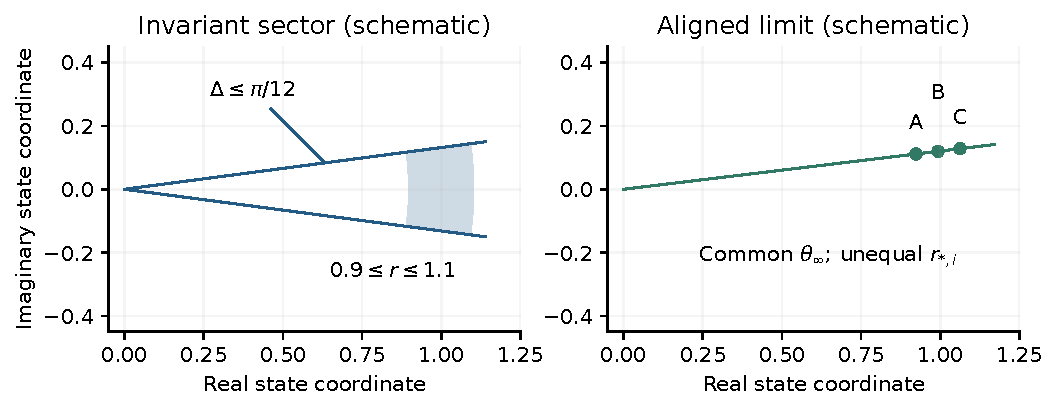
\includegraphics[width=\textwidth]{figures/sector_and_limit.pdf}
\caption{Schematic of the invariant sector and an aligned unequal configuration. Illustrated limiting radii are deliberately separated for visibility; they are not computed values of $r_*$. No trajectory or capture from the turning entrance is represented.}
\end{figure}

The observable consequences are immediate but distinct. If $\bar r_*=(1/3)\sum_i r_{*,i}$, then
\begin{equation}
m_n\to e^{i\theta_\infty}\bar r_*,\qquad
E_n\to E_*:=\|Pr_*\|_2>0.\label{eq:limits}
\end{equation}
For strict positivity, if $r_*=a\one$ with $a>0$, the graph part of \eqref{eq:fixed} vanishes and all three equations require $k_i=a^2$, contradicting the unequal coefficients. The same argument by subtracting two fixed equations excludes equal radii for a pair of distinct $k_i$. The actual limiting spread is fixed by the unique profile, and \eqref{eq:residual} bounds it above: $0<E_*\le C_{\rm disp}<0.005270$. It does not make the quoted upper bound an exact limiting value.

The full-state estimate also gives $|m_n-e^{i\theta_\infty}\bar r_*|\le d_n$ and $|E_n-E_*|\le\sqrt3d_n$. For cyclic $(i,j,k)$,
\begin{equation}
C_{i,n}=r_{j,n}r_{k,n}\sin(\theta_{k,n}-\theta_{j,n}),
\qquad |C_{i,n}|\le1.1^2\Delta_0c^n.\label{eq:Cdecay}
\end{equation}
Consequently $C_n\to0$, $W_n\to0$, and $\Gamma_n\to0$. Residual spread and signed area measure different features: unequal collinear complex vectors have nonzero dispersion and zero area.

There is no nonconstant periodic orbit entirely in $\mathcal D$, because every orbit there converges. Nor is there a nontrivial common-phase relative-periodic orbit: if $F^p(\Omega)=h\Omega$ with $|h|=1$, regular equivariance gives $F^{jp}(\Omega)=h^j\Omega$. Its nonzero limit forces $h=1$, and a convergent periodic sequence is constant. This excludes persistent ordinary relative phase rotation and sustained nonvanishing common-phase drift in this domain. It does not establish that each transient mean path is straight, or that it has only finitely many diminishing directional changes.

\section{Relation to the accepted fixed branch and other dynamics}\label{sec:prior}

The accepted response analysis already gives local attraction to the homogeneous fixed circle under strict normal stability and a nearby analytic positive branch for weak unequal coefficients \cite{response}. For the homogeneous triad at the present $\eps,g,\lambda$, the amplitude multipliers are $0.8,0.75,0.75$ and the two noncommon phase multipliers are $(1-3g)(1-9\lambda)=0.9215$. The common phase multiplier is one. These satisfy the accepted local hypotheses, but those hypotheses do not by themselves supply the explicit domain $\mathcal D$.

To identify the new domain theorem's fixed profile with continuation of the accepted unequal branch, consider
\begin{equation}
k(t)=\one+t(-0.001,0,0.001),\qquad0\le t\le1.\label{eq:continuation}
\end{equation}
Every amplitude-map bound used above holds uniformly along this interval. Each $\mathcal A_t$ has a unique interior fixed point $r_*(t)$, and $r_*(0)=\one$. Since $\|D\mathcal A_t\|_\infty\le\beta<1$, the matrix $I-D\mathcal A_t$ is invertible throughout. The analytic implicit-function theorem produces local branches, which uniqueness joins along the whole interval. Near zero this is the already accepted branch; at $t=1$ it is the profile in Theorem~\ref{thm:convergence}. This argument supplies the continuation that an unspecified local neighborhood could not supply on its own. It does not require a numerical continuation run or a root solve.

The contribution is an explicit finite domain of convergence with quantitative decay estimates, not a new equilibrium mechanism. The accepted positive-triad spectral result concerns real transverse quotient multipliers near aligned profiles \cite{spectral}. A bent finite nonlinear mean path does not contradict that local spectral statement, and it is not evidence for a missing complex linear mode.

The common-phase drift result concerns a different, twisted chiral relative-equilibrium branch. Its continuation starts from $2^{-1/2}e^{2\pi i j/3}$ and has a nonzero cubic-in-heterogeneity drift on the specified branch; its reference is a saddle, not a demonstrated attractor \cite[labels D1--D4 and D39--D45]{drift}. That state lies outside the narrow ordinary phase sector. The exclusion of persistent drift in $\mathcal D$ therefore does not exclude the accepted drift elsewhere at documented coefficients.

Paper G's certified alternating cycle likewise has a different entrance, parameter setting, and trapping certificate \cite{paperG}. Its retained area observables alternate rather than decay. Its local onset branch and its accepted finite capture are themselves carefully separated in that source. The present manuscript neither reopens those certificates nor asserts a continuation between that cycle, the twisted drift branch, and the aligned fixed circle. State-domain and parameter qualifications are part of each result, not details that can be dropped when comparing pictures.

\section{Geometry of the balances and coefficient roles}\label{sec:roles}

For positive $g$, each graph correction is
\begin{equation}
b_i=g(L_3\Omega)_i=3g(m-\Omega_i),\qquad\sum_i b_i=0.\label{eq:graphgeometry}
\end{equation}
Its direction points from that channel toward the current channel mean. This gives a precise state-space meaning to one possible ``toward the center'' description. The complete update also contains onsite response and synchronization, so this direction alone does not determine the next channel displacement or a physical trajectory.

The zero-sum vector identity is weaker than a magnitude-addition statement. For example $b_C=-(b_A+b_B)$ implies $|b_C|\le|b_A|+|b_B|$. Equality requires $b_A$ and $b_B$ to lie on the same ray, allowing a zero vector as a degenerate case; then $b_C$ lies on the opposite ray. Without these collinearity and sign conditions, complex cancellation does not make two magnitudes sum to a third.

The phase kicks obey a separate exact balance,
\begin{equation}
\sum_i\delta_i=0,\label{eq:kickbalance}
\end{equation}
because the sine contribution of every ordered pair cancels its reverse. These are real numbers, not graph vectors. If two nonzero kicks share one sign and the third has the opposite sign, the opposite kick's magnitude equals the sum of the other magnitudes. Equation~\eqref{eq:kickbalance} is therefore another possible three-number relation, but the historical identification remains unresolved. Also, zero sum of kicks does not make $S_n$ zero: the exact exponentials in \eqref{eq:budget} are weighted by different prestage vectors.

Stationarity need not mean every operation individually vanishes. At an aligned unequal fixed state, the graph and onsite terms cancel channel by channel in \eqref{eq:fixed}; the phase stage then acts trivially. Because the radii are not all equal and $g>0$, the graph correction vector is nonzero, and so is its compensating onsite vector. Individual entries may vanish where a radius equals the channel mean, but simultaneous cancellation of the complete vectors remains the relevant balance.

Dividing \eqref{eq:fixed} by nonzero $\eps$ gives
\begin{equation}
r_i(k_i-r_i^2)+\frac g\eps(L_3r)_i=0,
\qquad\frac g\eps=\frac16.\label{eq:ratioforce}
\end{equation}
Thus $g/\eps$ is the relative graph/onsite strength in the stationary amplitude equation. The synchronization strength disappears from this equation because aligned phase differences give zero kicks. It remains relevant to the evolving states and to the contraction estimates. Common scaling of $\eps$ and $g$ preserves this stationary balance equation but generally changes the finite discrete update and its stability. It is not an invariance of the complete dynamics.

These observations answer the geometrical question without assigning remembered quantities prematurely. An internal redistribution can be directed toward the mean, sum to zero, and still alter a later mean step after passing through nonlinear channel responses. A coherent limit can retain unequal radii while every area observable vanishes. Neither fact selects a unique spatial core coordinate from the accepted family of geometric observables \cite{closure}.

\section{Focused comparison with physical force laws}\label{sec:physics}

The relevant comparison with Newtonian attraction is structural and conditional. For noncolliding point masses $M_a>0$ at physical positions $\mathbf x_a(\tau)$ in an inertial frame, the Newtonian model is
\begin{equation}
M_a\frac{d^2\mathbf x_a}{d\tau^2}
=G_{\rm N}\sum_{b\ne a}M_aM_b
\frac{\mathbf x_b-\mathbf x_a}{|\mathbf x_b-\mathbf x_a|^3}.
\label{eq:newton}
\end{equation}
This is the point-particle inverse-square law in its classical regime, with physical time $\tau$ and Newton's dimensional constant $G_{\rm N}$ \cite{newton}. The direction toward another position can be compared with \eqref{eq:graphgeometry}. The graph correction, however, is linear in channel differences, with no inverse-distance factor or inertial state. Contracting channel dispersion therefore does not establish gravitational attraction. An actual correspondence would need a position map, a time calibration, inertial variables, physical units, and a justified response law. In particular $g$ has not been identified with $G_{\rm N}$.

For a classical nonrelativistic particle of mass $M$ and charge $q_{\rm el}$ in prescribed electric and magnetic fields, neglecting other forces and radiation reaction, the comparison equation is
\begin{equation}
M\frac{d^2\mathbf x}{d\tau^2}
=q_{\rm el}\left[\mathbf E_{\rm phys}(\mathbf x,\tau)
+\frac{d\mathbf x}{d\tau}\times\mathbf B_{\rm phys}(\mathbf x,\tau)\right].
\label{eq:lorentz}
\end{equation}
The electric force is $q_{\rm el}\mathbf E_{\rm phys}$ and the magnetic force is the velocity cross product with the field \cite{electric,magnetic}. The latter is perpendicular to velocity; its instantaneous power vanishes because $\mathbf v\cdot(\mathbf v\times\mathbf B_{\rm phys})=0$. These statements concern physical velocity and force, not consecutive complex increments.

The native turning statistic supplies neither acceleration in physical time nor an independently specified charge or field. It also combines direction and increment length, as the graph comparison demonstrates. Its nonzero value cannot establish a Lorentz response. Although $W$ has the accepted axial transformation law under the specified geometry, axial covariance alone does not supply magnetic units, a source equation, or a force on another degree of freedom. Identifying $\lambda$ with a magnetic field, or $W$ with a measured field, would add a model correspondence absent from the present results.

The comparison is useful because it makes the missing interfaces explicit. A future physical interpretation would have to connect native observables to measured variables and demonstrate the corresponding evolution law, including dimensions and operational meaning. This manuscript establishes state-space turning and relaxation at fixed mathematical coefficients. It does not infer those additional correspondences from visual similarity or from the word ``center.''

\section{SRG context and remaining programme interfaces}\label{sec:srg}

The author's interest in the product $\pi e\varphi\approx13.81758$, where $\varphi=(1+\sqrt5)/2$, remains part of the programme's motivation. The completed Final Mathematical Bridge identifies its documented role in the coupling construction
\begin{equation}
\gamma_*\,\pi e\varphi=\zeta(3),\qquad
\gamma_*=\frac{\zeta(3)}{\pi e\varphi}.\label{eq:srg}
\end{equation}
The bridge distinguishes historical associations of geometry, growth, packing, and discrete sums from a uniquely determined parameter-selection law. Its spectral reconstruction obtains the same coupling after a declared normalization and calibration; that later reconstruction is not presented as the original historical derivation \cite[\S6, equation S7]{bridge}. Missing historical motivations remain unrecovered motivations, not proof that the equations were arbitrary or invalid.

The bridge also distinguishes several meanings of REFU, TGMO, and RPCO across matrix operators and later recurrence implementations. The present paper inherits the specified native triad, not an unspecified synthesis of those historical systems. The coupling $\gamma_*$ is neither the fixed gain exponent appearing in another operator nor an independently measured physical coupling. Equations~\eqref{eq:parameters} are documented native coefficients; the present proofs do not derive them from $\pi e\varphi$, fit them to that product, or establish a physical connection to calendars or accelerators.

Several broader research interfaces remain visible without becoming assignments here. Natural core motion requires a justified core-position observable and its dynamics; the accepted observable census leaves more than one candidate. Gravity--magnetism comparisons require the missing physical correspondences described in Section~\ref{sec:physics}. Central $Z$ transport and the outer geometric structure require explicit choices about what is transported and whether the geometry is passive or dynamical. Legitimate SRG integration requires preserving source-specific operator meanings and any normalization or preparation assumptions. The TORMENT, intelligence, and embodiment programme remains a separate line of work rather than a consequence of the present triad theorem. Three-Way remains parked.

The unresolved recollection also remains an open historical interface. The exact graph and kick balances explain how a three-number relation could occur, but no retained equation identifies the remembered values. The selected turning entrance is deliberately not used to fill that gap. Likewise, no capture theorem is inserted between the finite turning witness and the coherent-domain theorem. Keeping these interfaces visible preserves the original questions while making the completed answers assessable.

\section{Evidence, scope, and review disposition}\label{sec:evidence}

\begin{table}[htbp]\centering\small
\caption{Results, parameter slices, domains, and evidence types.}
\begin{tabularx}{\textwidth}{@{}L{.22\textwidth}L{.21\textwidth}YY@{}}\toprule
Result & Coefficients & State domain & Evidence\\\midrule
Full-map turning and shape change & Equation~\eqref{eq:parameters} & One entrance, two updates & Retained rigorous intervals plus exact ratio.\\
Delayed graph response & Same $\eps,k$, $\lambda=0$; formal real $g$ & Fixed entrance; general polynomial identity & Exact algebra; retained rational check at $0,1/60$.\\
Invariant-domain spread bound & Full coefficients & Annulus and ordinary sector $\mathcal D$ & Analytical proof; retained constant enclosures.\\
Convergence and area decay & Full coefficients & Every state in $\mathcal D$ & Analytical theorem and explicit estimates.\\
Branch identification & Path \eqref{eq:continuation} & Unique profiles in $\mathcal Q$ & Uniform contraction and implicit-function theorem.\\
Historical number identification & Unspecified historical display & Not recovered & Author recollection; unresolved.\\\bottomrule
\end{tabularx}
\end{table}

The source baseline is the pinned commit shown on the cover. The eight cited project-source files were checked against that commit. All six named retained checker/receipt files were located and copied unchanged into \path{evidence/}; their origins and SHA-256 hashes are in \path{evidence/PROVENANCE.json}. Portable references in this package point to those copies, rather than to the original machine-local visualization directory.

The witness receipt supports a bounded computer-assisted nonzero claim. Its script is included so the arithmetic method can be inspected, not as a claim that it was executed again. The delayed-response receipt stores exact fractions and formal-polynomial checks. The domain receipt checks constants only, with zero state updates; the proof is the analytical argument above. The full convergence theorem needs neither a trajectory nor a computed root. These distinctions prevent a build receipt or a diagram from being mistaken for new mathematical certification.

The preparation pass generated figures from retained values and a labelled schematic, transcribed the completed proofs, checked references and formulas, and built and inspected the PDF. Publication finalization applied the two approved wording clarifications and edition-status updates, then rebuilt and inspected the document. Neither pass changed the native or production kernels, reran completed simulations, or broadened the interval certificate. The original archival scripts retain their local-path assumptions and safety assertions; they are not run by the manuscript build. The historical review handoff records preparation checks and editorial evidence limitations; \path{PUBLICATION_DISPOSITION.md} records the completed reviews, publication authorization, and final document checks.

This is the author-authorized repository research edition v0.1, with GPT project-internal scientific review and author review completed on 28 October 2026. No external peer review is claimed. The mathematical conclusions are bounded: internal redistribution can redirect later collective evolution through nonlinear response, and separately an explicit region relaxes to unequal alignment. Sustained motion, physical magnetism, a completed gravitational theory, historical numerical identification, and capture of the turning entrance are not established by these results.

\appendix
\section{Retained stage budgets and certificate interpretation}\label{app:budgets}

The following enclosures are read directly from the retained witness receipt, using the same contribution definitions as \eqref{eq:budget}. They show where the realized mean change enters at each of the two updates. They do not separate the graph's indirect influence on the input state from later onsite evaluation; that question is addressed by the matched comparison instead.
\begin{table}[htbp]\centering\footnotesize
\caption{Onsite and synchronization contributions in the full-map witness.}
\begin{tabular}{@{}llll@{}}
\toprule
$n$ & Contribution & Real part & Imaginary part \\
\midrule
0 & $B_n$ & $[-0.2000000001, -0.1999999999]$ & $[0.1998999999, 0.1999000001]$ \\
0 & $S_n$ & $[-0.0031076834, -0.0031076833]$ & $[0.0004797848, 0.0004797849]$ \\
1 & $B_n$ & $[-0.0431887973, -0.0431887972]$ & $[-0.0093260456, -0.0093260455]$ \\
1 & $S_n$ & $[-0.0031331047, -0.0031331046]$ & $[0.0004927978, 0.0004927979]$ \\
\bottomrule
\end{tabular}

\end{table}

The original certificate represents intervals by integer endpoints divided by $2^{200}$. Square-root endpoints are bounded by integer square roots. With $u_i=v_i/|v_i|$, the identity
\[
\sin3(\operatorname{Arg}v_j-\operatorname{Arg}v_i)=\im[(u_j\bar u_i)^3]
\]
avoids choosing a different angle branch. The exponential uses sine through degree 19 and cosine through degree 20; for $|\delta|<1/100$, the absolute remainder bounds are $(1/100)^{21}/21!$ and $(1/100)^{22}/22!$, respectively. Outward rounding encloses the rational operations as well. The short decimal intervals in the text are coarser, readable consequences of the stored exact endpoints.

The phase-off control uses exact rational arithmetic. Conjugation is established by symmetry rather than a second computed path. No claims are made about arbitrary long floating-point realizations: the manuscript's theorems concern the exact recurrence, and the certificate encloses just the stated finite witness.

\section{Exact coefficients of the prescribed graph comparison}\label{app:coefficients}

For the entrance in \eqref{eq:entrance}, the fixed $\eps,k$ of \eqref{eq:parameters}, and $\lambda=0$, the retained arrays are
\begin{align}
a&=\left(\frac{8999}{10000}(1+i),\frac9{10}(1+i),
                 \frac{6001}{10000}(1-2i)\right),\\
d&=(-3i,-3i,6i).
\end{align}
The polynomial coefficients in \eqref{eq:poly} are
\begin{align}
P_1&=\frac{61206001}{100000000}-i\frac{144042011}{500000000},\\
P_2&=-\frac{126009}{100000}+i\frac{270081}{100000},
\qquad P_3=-\frac{27}{5}i.
\end{align}
The first-order split and its evaluated comparison are
\begin{align}
P_{1,k}&=\frac3{10000}i,
&P_{1,\rm cub}&=\frac{61206001}{100000000}-i\frac{144192011}{500000000},\\
g_*P_{1,k}&=\frac{i}{200000},
&D_{\rm cub}(g_*)&=\frac{59105851}{6000000000}-i\frac{122435261}{30000000000}.
\end{align}
Adding the two evaluated parts recovers \eqref{eq:Dstar}. The corresponding signed-turn comparison is
\begin{align}
K(0)&=\frac{1168259827345999}{100000000000000000},\\
K(g_*)&=\frac{3158587023292997}{300000000000000000},\\
J(g)&=-\frac{64733991599}{1000000000000}g
      -\frac{288270009}{1000000000}g^2+\frac{27}{25}g^3.
\end{align}
The \href{evidence/delayed_graph_response_20261028.json}{graph-response receipt} also retains the exact coefficients of $R(g)$ and of $Q(g)-|t(0)|^2$, under the keys \path{R_coefficients} and \path{direction_dot_coefficients}, respectively. The nonzero constant term of $Q(g)$ must therefore be added when evaluating that diagnostic. Their sign evaluation is stated in \eqref{eq:signs}; no parameter sweep is implied by storing the formal polynomial.

\section{Source and attribution notes}\label{app:sources}

The bibliography links project sources to the fixed commit, so later repository changes do not silently change this edition's mathematical baseline. The claim/source map distinguishes inherited definitions, inherited local theorems, newly completed propositions, existing computational evidence, author recollections, and unresolved interpretations. The preparation order is preserved as provenance for the requested account of the observation and review sequence; it is not an independent scientific validation.

All six specifically requested retained files were available. No separate standalone transcript of the optional earlier onsite-only fixed-channel-phase example was located among those retained files, so that optional example is not reconstructed or presented as recovered evidence. The manuscript's mechanism distinction instead uses the supplied exact matched comparison and the definitions of $K,J,R,Q$. This omission does not remove any of the required positive results or their qualifications.

Hilmir Fr\'imann Halld\'orsson supplied the research observation, questions, and programme direction. GPT supplied scientific steering and project-internal review of the completed mathematical reports and this assembled manuscript. Codex supplied mathematical and computational assistance in that investigation and prepared the present source-linked synthesis, figures, and publication materials. GPT scientific review and author approval were completed on 28 October 2026, and the author authorized repository publication. Internal AI-assisted review is not external peer review; responsibility for author approval and publication remains with the author. No DOI, journal placement, new Paper A--G letter, or external review status is assigned.

\begin{thebibliography}{99}\small
\bibitem{kernel} Tri-Octagon project, \emph{Native deterministic recurrence}, \texttt{kernel\_physics/dynamics.py}, especially \texttt{arg0}, \texttt{phase\_sync}, and \texttt{\_advance}. \href{https://github.com/pzychozen/trioctagon-physics/blob/ad8a6e88b4a78d8b1955b34d5ff80b6c21713ade/kernel_physics/dynamics.py}{Pinned implementation}.
\bibitem{paperA} H. F. Halld\'orsson, \emph{Cycle-Covering Dynamics of a Three-State Nonlinear Kernel}, Paper A publication edition, \S1 and \S6.1. \href{https://github.com/pzychozen/trioctagon-physics/blob/ad8a6e88b4a78d8b1955b34d5ff80b6c21713ade/papers/PAPER_A/publication/paper_A_publication.md}{Pinned manuscript}.
\bibitem{response} Tri-Octagon project, \emph{Native Response Geometry and Spectral Circulation in the Tri-Octagon Map}, v0.1, response chapter: ``Homogeneous finite-ring response'' and ``Weak unequal-background branch.'' \href{https://github.com/pzychozen/trioctagon-physics/blob/ad8a6e88b4a78d8b1955b34d5ff80b6c21713ade/papers/NATIVE_RESPONSE_GEOMETRY/manuscript/response.tex}{Pinned chapter source}.
\bibitem{spectral} Same work, spectral chapter: ``Exact positive-triad spectrum.'' \href{https://github.com/pzychozen/trioctagon-physics/blob/ad8a6e88b4a78d8b1955b34d5ff80b6c21713ade/papers/NATIVE_RESPONSE_GEOMETRY/manuscript/spectral.tex}{Pinned chapter source}.
\bibitem{closure} Same work, observables and closure chapter: ``Equivariant spatial observables,'' ``Chiral projections and native observable changes,'' and ``The essential zero-stratum exception.'' \href{https://github.com/pzychozen/trioctagon-physics/blob/ad8a6e88b4a78d8b1955b34d5ff80b6c21713ade/papers/NATIVE_RESPONSE_GEOMETRY/manuscript/observables_closure.tex}{Pinned chapter source}.
\bibitem{drift} H. F. Halld\'orsson, \emph{Cubic Common-Phase Drift on a Chiral Branch of the Tri-Octagon Map}, v0.1, 6 October 2026, labels D1--D4 and D39--D45. \href{https://github.com/pzychozen/trioctagon-physics/blob/ad8a6e88b4a78d8b1955b34d5ff80b6c21713ade/papers/MEASUREMENT_AND_CHIRAL_DRIFT/v0.1/drift/manuscript.tex}{Pinned manuscript source}.
\bibitem{paperG} H. F. Halld\'orsson, \emph{Paper G: Geometry-Attached Axial Observables}, v0.1.1, 4 October 2026, definitions \texttt{eq:SA}, \texttt{eq:T}, \texttt{eq:W}, and the accepted alternating-cycle discussion. \href{https://github.com/pzychozen/trioctagon-physics/blob/ad8a6e88b4a78d8b1955b34d5ff80b6c21713ade/papers/PAPER_G/v0.1.1/source/paper_g.tex}{Pinned manuscript source}.
\bibitem{bridge} \emph{SRG Final Mathematical Bridge: From Lens Geometry to Recurrence and Known Equations}, accepted publication edition v0.1, prepared for H. F. Halld\'orsson, 27 October 2026, \S\S3,5--7, especially equation S7. \href{https://github.com/pzychozen/trioctagon-physics/blob/ad8a6e88b4a78d8b1955b34d5ff80b6c21713ade/SRG_REDISCOVERY/FINAL_MATHEMATICAL_BRIDGE/publication/v0.1/SRG_FINAL_MATHEMATICAL_BRIDGE_v0.1.md}{Pinned publication}.
\bibitem{turnreceipt} Codex-assisted completed investigation, \emph{Two-step turning witness and phase-off control}, retained 28 October 2026. \href{evidence/turning_witness_20261028.json}{Exact interval receipt}; \href{evidence/turning_witness_20261028.py}{archival checker}. Copied unchanged, not rerun for this draft.
\bibitem{graphreceipt} Codex-assisted completed investigation, \emph{Delayed graph response}, retained 28 October 2026. \href{evidence/delayed_graph_response_20261028.json}{Exact rational receipt}; \href{evidence/delayed_graph_response_20261028.py}{archival checker}. Copied unchanged, not rerun for this draft.
\bibitem{domainreceipt} Codex-assisted completed investigation, \emph{Moving-mean domain constants}, retained 28 October 2026. \href{evidence/moving_mean_domain_constants_20261028.json}{Constant-enclosure receipt}; \href{evidence/moving_mean_domain_constants_20261028.py}{archival constant checker}. Analytical proof support only; no state updates. Copied unchanged, not rerun for this draft.
\bibitem{order} \emph{Tri-Octagon Physics: Manuscript Preparation Work Order}, GPT-written order supplied and invoked by the author, 28 October 2026. \href{evidence/MANUSCRIPT_WORK_ORDER.txt}{Unchanged supplied text}. Source for the recollection, scope, and review sequence; not independent validation.
\bibitem{newton} OpenStax, \emph{University Physics}, Volume 1, \S13.1, ``Newton's Law of Universal Gravitation.'' \href{https://openstax.org/books/university-physics-volume-1/pages/13-1-newtons-law-of-universal-gravitation}{Publisher textbook section}, consulted 28 October 2026.
\bibitem{electric} OpenStax, \emph{University Physics}, Volume 2, \S5.4, ``Electric Field.'' \href{https://openstax.org/books/university-physics-volume-2/pages/5-4-electric-field}{Publisher textbook section}, consulted 28 October 2026.
\bibitem{magnetic} OpenStax, \emph{University Physics}, Volume 2, \S11.2, ``Magnetic Fields and Lines.'' \href{https://openstax.org/books/university-physics-volume-2/pages/11-2-magnetic-fields-and-lines}{Publisher textbook section}, consulted 28 October 2026.
\end{thebibliography}

\end{document}
